\documentclass[xcolor={table}]{beamer}

% Packages
\usepackage[brazil]{babel}	
\usepackage[utf8]{inputenc}
\usepackage[T1]{fontenc}
\usepackage[scaled]{helvet}
\usepackage{amsthm}
\usepackage{ragged2e}
\usepackage{subfig}
\usepackage[table]{xcolor}
\usepackage{multicol}
\usepackage{multirow}
\usepackage{fancyvrb}
\usepackage{verbatim}
\usepackage{minted}

% Configuration for packages
\usemintedstyle{bw}

% Theme
\usetheme{Execushares}

% Title page configuration
\title{Laborator III: \textit{Shellcodes} II. Atacuri cu Șiruri de Caractere de Formatare}
\subtitle{}
\author{Iosif George-Andrei}
\setcounter{showSlideNumbers}{1}

\begin{document}

    % Title page
    \setcounter{showProgressBar}{0}
	\setcounter{showSlideNumbers}{0}
	\frame{\titlepage}

    % Table of content
	\begin{frame}
		\frametitle{Tabelă de Conținut}\pause
		\begin{enumerate}[<+->]
			\item Atacuri cu Șiruri de Caractere de Formatare
			\item Exemplu Concret
		\end{enumerate}
	\end{frame}

    % First section
	\setcounter{framenumber}{0}
	\setcounter{showProgressBar}{1}
	\setcounter{showSlideNumbers}{1}
	\section{Atacuri cu Șiruri de Caractere de Formatare}

	\begin{frame}
		\frametitle{Funcționalitate de Formatare}\pause
		\begin{itemize}[<+->]
		    \item Prezența unor funcționalități de formatare în majoritatea limbajelor de operare (inclusiv în domeniul \textit{web})
			\item Pentru C, suport oferit prin:
			    \begin{itemize}
			        \item Funcții specifice
			        \item Șiruri de caractere de formatare
			        \item Parametrii
			    \end{itemize}
		\end{itemize}
	\end{frame}
	
	\begin{frame}
		\frametitle{Funcții Specifice în C}\pause
		\begin{itemize}[<+->]
			\item \mintinline{bash}{printf}: Scrie formatat la \mintinline{bash}{stdout}.
			\item \mintinline{bash}{fprintf}: Scrie formatat într-un fișier.
			\item \mintinline{bash}{sprintf}: Scrie formatat într-un șir de caractere.
			\item \mintinline{bash}{snprintf}: Scrie formatat într-un șir de caractere, ținând cont și de lungimea maximă.
		\end{itemize}
	\end{frame}
	
	\begin{frame}
		\frametitle{Șiruri de Caractere de Formatare. Parametrii}\pause
		\begin{itemize}[<+->]
		    \item \textbf{Șiruri de Caractere de Formatare}: Șir de caractere format din text propriu-zis (ce va fi scris ca atare) și din parametrii (identificați prin \textbf{\%})
		    \item Exemple de parametrii
    	        \begin{itemize}
    		        \item \textbf{\mintinline{bash}{d}}: Scrie în format zecimal valoarea primită ca parametru.
    		        \item \textbf{\mintinline{bash}{x}}: Scrie în format hexazecimal valoarea primită ca parametru.
    		        \item \textbf{\mintinline{bash}{s}}: Dereferențiază adresa primită ca parametru și scrie șirul de caractere (terminat în \mintinline{bash}{NULL}) găsit acolo.
    		        \item \textbf{\mintinline{bash}{n}}: Populează o zonă de memorie primită ca parametru cu numărul de caractere ce au fost scrise.
    		    \end{itemize}
		\end{itemize}
	\end{frame}
	
	\begin{frame}
		\frametitle{Atacuri cu Șiruri de Caractere de Formatare}\pause
		\begin{itemize}[<+->]
		    \item Presupun injectarea unui astfel de șir de caractere într-o funcție.
		    \item Asemănător injectării în șabloane la nivel de server (engl. "\textit{server-side template injection}" și abreviat SSTI)
		\end{itemize}
	\end{frame}
	
	\begin{frame}
		\frametitle{Rezultatele Atacurilor}\pause
		\begin{itemize}[<+->]
		    \item Citirea informației din memoria procesului
			\item Modificarea informației din memoria procesului
		\end{itemize}
	\end{frame}
	
	\begin{frame}
		\frametitle{Protecții împotriva Atacurilor}\pause
		\begin{itemize}[<+->]
			\item Sanitizarea intrărilor de la utilizator
			\item Activarea avertizărilor și a protecțiilor, la nivel de compilator
		\end{itemize}
	\end{frame}

	% Second section
	\section{Exerciții}

	\begin{frame}
		\frametitle{Recomandări}\pause
		\begin{itemize}[<+->]
		    \item Folosiți comanda \mintinline{bash}{man} pentru a primi ajutor la rularea anumitor comenzi.
		    \item Folosiți \href{https://docs.pwntools.com/en/stable/}{documentația \mintinline{bash}{pwntools}} pentru a identifica metodele de care aveți nevoie.
	    \end{itemize}
	\end{frame}

    % Third section
	\section{\textit{Exemplu Concret}}

	\begin{frame}
		\frametitle{Atacuri în Sistemele Multimedia ale Mașinilor I}\pause
		\begin{figure}
            \centering
            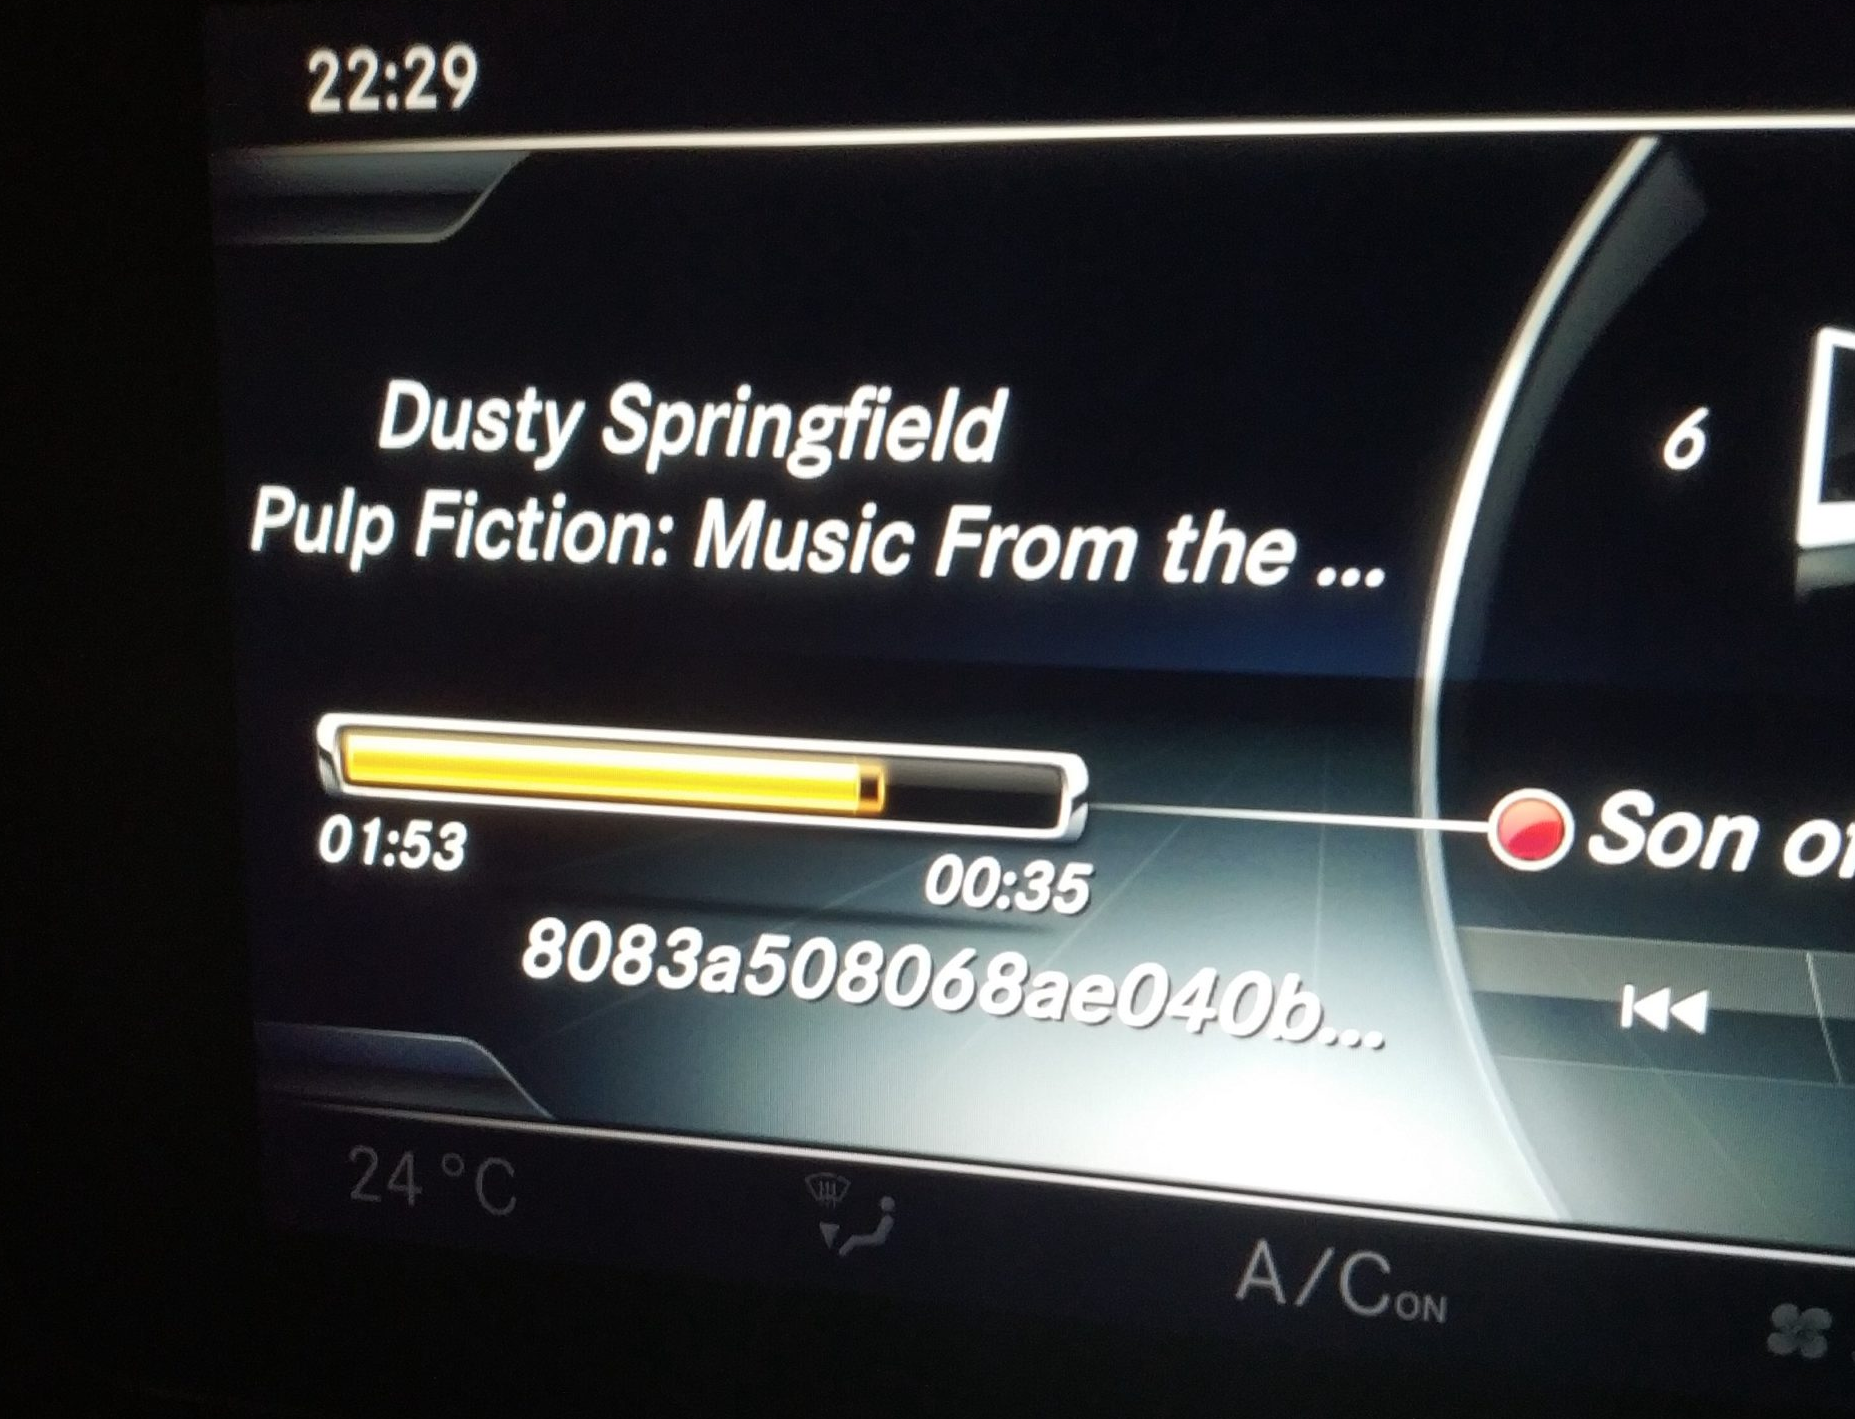
\includegraphics[width=8cm]{images/automotive.png}
        \end{figure}
    \end{frame}

	\begin{frame}
		\frametitle{Atacuri în Sistemele Multimedia ale Mașinilor II}\pause
		\begin{itemize}[<+->]
		    \item Multiple vulnerabilități la atacuri cu șiruri de caractere de formatare, găsite în sistemele multimedia ale unor mașini
		    \item Numele dispozitivului conectat ca vector de atac
		    \item Mai multe mașini găsite ca fiind vulnerabile ca urmare a unei postări inițiale pe \href{https://twitter.com/0xRaindrop/status/864704956116254720}{Twitter}
    		    \begin{itemize}
    			    \item BMW 330i 2011
    			    \item Camioane GMC 2016
    			    \item Audi A7 2014 
    			\end{itemize}
		\end{itemize}
	\end{frame}

    % Forth section
	\section{Recapitulare}

	\begin{frame}
		\frametitle{Recapitulare}\pause
		\begin{figure}
            \centering
            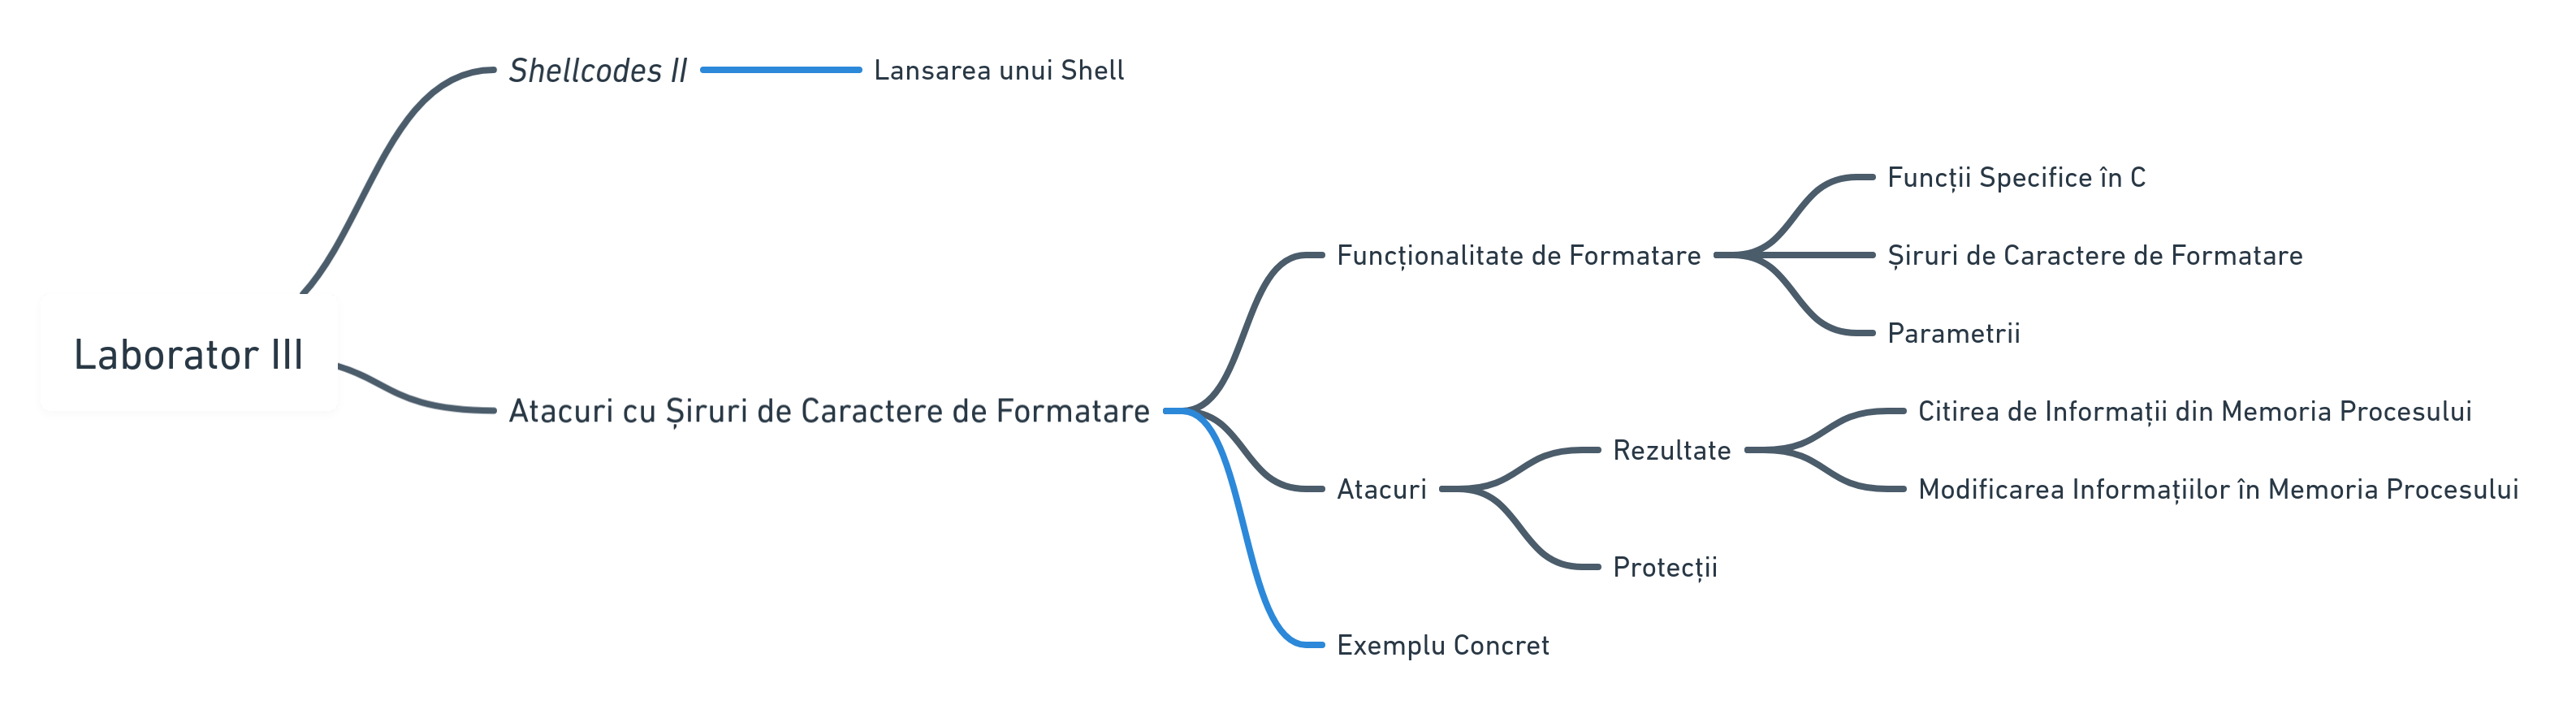
\includegraphics[width=11cm]{images/recap.png}
        \end{figure}
	\end{frame}

\end{document}